\chapter{Metodologia}
\label{cap:metodologia}

Este capítulo apresenta os procedimentos adotados para condução da pesquisa, abrangendo o tipo de abordagem, o problema de pesquisa, os objetivos, as hipóteses consideradas, o referencial teórico utilizado, os métodos de coleta de dados e o planejamento da análise.

\section{Tipo de Pesquisa}

A presente pesquisa pode ser caracterizada como \textbf{aplicada}, pois visa o desenvolvimento de uma solução prática para um problema real, por meio da criação de um aplicativo para auxiliar na gestão de propriedades rurais. A abordagem metodológica adotada é \textbf{quali-quantitativa}, combinando a análise qualitativa das percepções dos usuários com dados quantitativos obtidos através de questionários estruturados. Neste contexto, optou-se por utilizar a \textbf{pesquisa de levantamento}, a qual possibilita a coleta de dados de uma amostra representativa da população-alvo, permitindo identificar padrões, dificuldades recorrentes e necessidades específicas relacionadas à gestão rural.

\section{Problema de Pesquisa}

A questão norteadora desta pesquisa é: \textit{Como melhorar a gestão da produção em pequenas e médias propriedades rurais por meio de software?}

\section{Etapas do projeto}

\subsection{Etapa 1 - Levantamento de necessidades dos produtores}

Realizar uma pesquisa para identificar as principais dificuldades enfrentadas pelos proprietários de fazendas em relação à gestão de suas propriedades. Essa investigação tem como objetivo compreender as demandas mais recorrentes no campo, envolvendo aspectos como controle de rebanho, uso de insumos, registros sanitários e organização financeira, permitindo a definição de requisitos relevantes para o sistema.

\subsection{Etapa 2 - Projeto da interface do usuário}

Projetar uma interface de usuário simples e acessível, adequada para produtores com diferentes níveis de familiaridade com tecnologia. A interface será desenvolvida com foco na clareza visual, ²facilidade de navegação e acessibilidade, de forma a garantir que qualquer usuário, independentemente de sua experiência com dispositivos móveis, consiga utilizar o sistema de maneira autônoma e eficiente.

\subsection{Etapa 3 - Implementação de funcionalidades de controle animal}

Implementar funcionalidades que permitam o registro e acompanhamento do histórico dos animais, produção de leite e controle de vacinação. O módulo será responsável por organizar informações essenciais sobre cada animal, possibilitando ao produtor acompanhar dados como nascimento, peso, doenças, vacinação e rendimento produtivo, auxiliando na tomada de decisões relacionadas ao manejo.

\subsection{Etapa 4 - Desenvolvimento do módulo de gestão de estoque}

Desenvolver um módulo de gestão de estoque para insumos, como rações, medicamentos, materiais de manejo e outros recursos utilizados na atividade pecuária. O sistema permitirá o controle de entrada e saída de materiais, alertando sobre níveis críticos de estoque e contribuindo para uma administração mais eficiente dos recursos.

\subsection{Etapa 5 - Implementação de projeções financeiras}

Desenvolver módulos que forneçam projeções financeiras, auxiliando na tomada de decisões estratégicas. Com base nas informações inseridas no sistema, o aplicativo poderá gerar relatórios e estimativas sobre custos operacionais, receitas e lucros, promovendo uma visão mais clara da situação econômica da propriedade e apoiando o planejamento de ações futuras.


\section{Hipóteses}

A hipótese central deste estudo é: \textit{Se os produtores tiverem acesso a um sistema de gestão intuitivo, então sua capacidade de planejamento e organização da produção será significativamente melhorada.}

\section{Coleta de Dados}

A coleta de dados será realizada por meio de um questionário online distribuído via Google Forms, conforme os princípios da pesquisa de levantamento. O público-alvo são produtores e funcionários de fazendas de pequeno porte no interior do Ceará, com faixa etária entre 18 e 40 anos — grupo considerado mais propenso à adoção de soluções tecnológicas. As perguntas foram elaboradas para identificar as principais dificuldades enfrentadas na gestão da produção, o grau de organização atual e o comportamento em relação ao uso de ferramentas digitais. Serão também utilizados dados secundários, como pesquisas do IBGE, para complementar o contexto da amostra.

\section{Análise de Dados}

Os dados coletados serão analisados por meio de técnicas de \textbf{análise estatística descritiva}, utilizando ferramentas como Microsoft Excel ou Google Sheets. As respostas fechadas serão tratadas por frequência e percentual, com representação gráfica em formatos de barras e pizza. As respostas abertas serão agrupadas por categorias temáticas, permitindo a identificação de padrões qualitativos. Esta análise embasará as decisões de projeto do aplicativo e a validação da hipótese proposta.
	\begin{figure}[h!]
		\centering
		\Caption{\label{fig:topicos_motodologia} Etapas da metodologia}	
		\UNIFORfig{}{
			\fbox{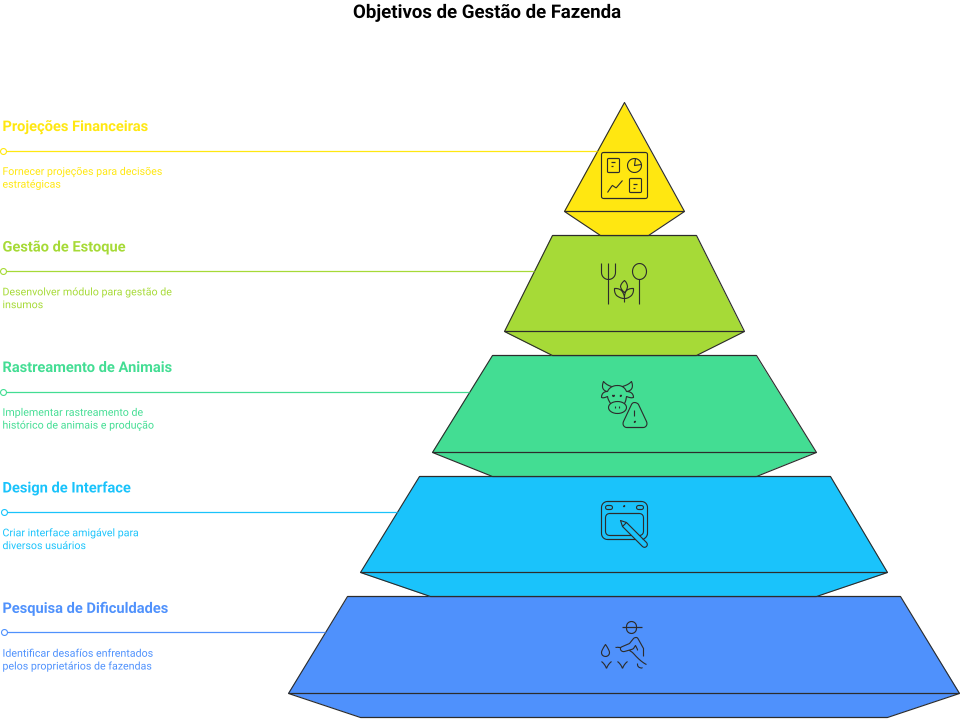
\includegraphics[width=10cm]{figuras/topicos_motodologia}}
		}{
			\Fonte{Elaborado pelo autor}
		}
	\end{figure}